\documentclass{article}
\usepackage{graphicx}
\usepackage[margin=1in]{geometry}
\usepackage{caption}
\usepackage{multirow}
\usepackage{array}
\usepackage{hyperref}
\usepackage{listings}
\graphicspath{ {./images} }
\title{Requirements And Specifications Document}
\author{
	Politecnico di Milano\\
	Merlino Lorenzo \& Iodice Andrea
}

\date{\today}
\begin{document}
\maketitle
\tableofcontents
\newpage
\section{Introduction}
\subsection{Purpose}
The System to Be will allow users to take part in coding battles. Each coding battle will be part of a tournament and consists of a coding project to be completed.
Educators will create tournaments and create battles by supplying the project structure. 
Students will be able to create teams and the teams will be able to submit a solution to the coding battle. Each solution will be scored using different criterias, such as the amount of test cases passed, amount of time required to submit the solution and quality of the code provided.
Some criteria will be automatically asserted and the remaining ones will be asserted by the creator of the battle.
\subsubsection{Goals}
The goals the system aims to achieve are:\\\\
\textbf{[G1]} Educator is able to create and manage a tournament.\\
\textbf{[G2]} Educator is able to allow other educators to manage their tournament.\\
\textbf{[G3]} Educator is able to create and manage code battles for a tournament they are involved in.\\
\textbf{[G4]} Any user is able to authenticate with their GitHub account. \\
\textbf{[G5]} Student is able to enroll in tournament and join/create a team.\\
\textbf{[G6]} Any Team participating in a battle is able to submit a solution.\\
\textbf{[G7]} Students are able to see their current rank and score in the tournaments they are taking part.\\
\textbf{[G8]} Educators are able to see Students’ current rank and score in the tournaments they are involved in.\\
\textbf{[G9]} Educators are able to assign a grade to solutions submitted by Teams subscribed to a Battle created by the Educator.\\
\subsection{Scope}
CodeKataBattle (CKB) is a new platform that helps students improve their software development skills by training with peers on code kata. 
\\\\
Educators use the platform to challenge students by creating code kata battles in which teams of students can compete against each other, thus proving and improving their skills. 
\\\\
Educators create tournaments to which students can enroll. After enrolling in a tournament students can take part in code kata battle by joining or creating a team.
\\\\
A code kata battle is a programming exercise.
The exercise includes a brief textual description and a software project with build automation scripts that contains a set of test cases that the program must pass.
\\\\
Teams participating in a battle are expected to follow a test-first approach and develop a solution that passes the required tests. Groups deliver their solution to the platform before the deadline.
At the end of the battle, the platform and the educators assign scores to groups, in order to create a competition rank.
\\\\
A Educator cannot be a student and vice versa.
\subsubsection{World Phaenomena}
Phenomena events that take place in the real world and that the machine cannot observe:\\\\
\textbf{[W1]} Educator wants to create a tournament\\
\textbf{[W2]} Educator wants to allow another educator to create battles in their tournament\\
\textbf{[W3]} Student wants to participate in a tournament\\
\textbf{[W4]} A team modifies their implementation of the solution\\
\textbf{[W5]} Student wants to check his rank\\
\textbf{[W6]} Student wants to join a team\\
\subsubsection{Shared Phaenomena world controlled}
Phenomena controlled by the world and observed by the machine:\\\\
\textbf{[SP1]} User logs in the system\\
\textbf{[SP2]} Educator creates a tournament\\
\textbf{[SP3]} Educator allows another educator to create battles for their tournament\\
\textbf{[SP4]} Educator creates a battle for their tournament\\
\textbf{[SP5]} Educator assign grade for a solution\\
\textbf{[SP6]} Educator closes a tournament\\
\textbf{[SP7]} Student joins tournament\\
\textbf{[SP8]} Student creates a team\\
\textbf{[SP9]} Student joins a team\\
\textbf{[SP10]} Student invites another student to the team\\
\textbf{[SP11]} Student checks is rank for a tournament they are participating in\\
\textbf{[SP12]} A team pushes their solution to GitHub\\
\textbf{[SP13]} Battle’s deadline is reached\\
\textbf{[SP14]} Student receives invite to a team\\
\subsubsection{Shared Phaenomena machine controlled}
Phenomena controlled by the machine and observed by the world:\\\\
\textbf{[SP15]} System notifies student they have been invited to a team\\
\textbf{[SP16]} System assign automatic grading\\
\textbf{[SP17]} System notifies students a new battle is available\\
\textbf{[SP18]} System notifies students a new tournament is available\\ 
\textbf{[SP19]} System notifies a tournament has been closed\\
\textbf{[SP20]} System notifies a student a battle is ended\\
\textbf{[SP21]} System notifies a team their solution has been graded\\
\textbf{[SP22]} System notifies educator that a new submission is ready to be graded\\
\textbf{[SP23]} System notifies student that the student they have invited to their team has accepted/rejected the invite.\\
\subsection{Definitions, Acronyms, Abbreviations}
\subsubsection{Definitions}
\begin{itemize}
\item \textbf{Coding Battle}: programming exercise proposed by an Educator in the context of a tournament.
\item \textbf{Tournament}: a series of coding battles, in which Students can take part as teams. It’s created and managed by an Educator.
\item \textbf{Team}: group of students who enroll in a tournament. Students in the same team work together and the solution they submit will be taken into consideration for each member of the team.
\item \textbf{Rank}: position of a Student in a tournament’s leaderboard, which is calculated on each Student’s score.
\item \textbf{Score}: points gained by a Student by submitting a solution to a Coding Battle.
\item \textbf{Open battle}: a battle that accepts new submissions.
\item \textbf{Closed battle}: a battle that doesn’t accept new submissions but some still need to be evaluated.
\item \textbf{Completed battle}: a battle that doesn’t accept new submissions and where all the submissions have been evaluated.
\item \textbf{Open tournament}: A tournament where new battles can be created.
\item \textbf{Closed tournament}: A tournament where new battles cannot be created but some are still not completed.
\item \textbf{Completed tournament}: A tournament where new battles cannot be created and all battle have been completed
\item \textbf{Team leader}: Student who created the team.
\item \textbf{Automated grading}: A series of scores that is automatically assigned to a solution, it is composed of:
\begin{itemize}
\item Number of test passed
\item Time passed after the battle publication
\item Static analysis result
\end{itemize}
\item \textbf{User}: either a Student or an Educator
\item \textbf{Educator}: user of the system, who manages tournaments and battles.
\item \textbf{Student}: user of the system, who participates in tournaments and battles.
\end{itemize}
\subsubsection{Acronyms}
\begin{itemize}
\item \textbf{RASD}: Requirements Analysis and Specification Document
\end{itemize}
\subsubsection{Abbreviations}
\begin{itemize}
\item \textbf{[Gn]}: the n-th goal of the system
\item \textbf{[Wn]}: the n-th world phaenomena
\item \textbf{[Rn]}: the n-th requirement
\item \textbf{[SPn]}: the n-th shared phaenomena
\item \textbf{[UCn]}: the n-th use case
\item \textbf{[SCn]}: the n-th scenario
\end{itemize}
\subsection{Revision History}
\begin{itemize}
\item Version 1.0
\end{itemize}
\subsection{Reference Documents}
\begin{itemize}
\item The specification of the RASD \&\& DD assignment of the Software Engineering II course, held by professors Matteo Rossi, Elisabetta Di Nitto and Matteo Camilli in Politecnico di Milano, A.Y. 2023/2024.
\item Slides of the Software Engineering II course on the WeBeep website.
\end{itemize}
\subsection{Document Structure}
This document is divided into 6 sections:\\
\begin{enumerate}
\item \textbf{Introduction}: it aims to describe the environment and the demands taken
into account for this project. In particular it’s focused on the reasons and the
goals that are going to be achieved with its development
\item \textbf{Overall Description} it’s a high-level description of the system by focusing on the shared phenomena and the domain model (with its assumption)
\item \textbf{Specific Requirements}: it describes in very detail the requirements needed
to reach the goals. In addition it contains more details useful for developers
(i.e information about HW and SW interfaces)
\item \textbf{Formal Analysis}: this section contains a formal description of the main
aspect of the World phenomena by using Alloy
\item \textbf{Effort Spent}: it shows the time spent to realize this document, divided for each section
\item \textbf{References}: it contains the references to any documents and to the Software
used in this document
\end{enumerate}

\newpage
\section{Overall Description}
\subsection{Product Perspective}
\subsubsection{Scenarios}
Note: \textit{ The login process will be handled by github. Moreover, these scenarios require that the user has done the login procedure.}

\paragraph{[SC1]}Educator creates a tournament:\\
An educator wants to create a new tournament. They log in into the system and access system tools to create a tournament. At this point the educator must define the tournament name and other educators that can create battles. If all the information has been inserted correctly the educator can confirm the creation of the tournament. The system will create the tournament and notify all the students.

\paragraph{[SC2]}Educator adds another educator in a tournament they manage:\\
An educator has created a tournament and wants to add another educator to it. The educator will ask the system for a list of all the tournaments they created, they select the one they are interested in, then they will ask the system the list of all the educators, select the ones they are interested in and confirm their choice, the system will signal whether the operation was successful or not. If the operation was successful the added educators will be notified that they can now create battles for this tournament.

\paragraph{[SC3]}Educator wants to create a battle:\\
An educator has either created a tournament or has been allowed to create battles for a tournament. The Educator logs into the system and will select a tournament they are managing. After that, the Educator asks the system to create a new battle for said tournament and specifies: the name of the battle, the minimum and maximum size of a team for this battle, the registration deadline, the submission deadline, the scoring configuration and the GitHub repository containing the description of the battle and the software project. The educator confirms the creation of the battle and, if all the information is valid, the battle is created and all the students enrolled in the tournament are notified of the new battle.

\paragraph{[SC4]}Educator assign grade for a solution:\\
The educator logs into the system and asks the system for a list of all the submissions ready to be graded. The educator selects the submission they want to grade, review the submission and assign a grading according to the grading configuration. The grading is recorded in the system and the students are notified.

\paragraph{[SC5]}Educator closes a tournament:\\
The educator wants to close a tournament, they ask the system for a list of all the open tournaments the Educator is managing. The educator selects the tournament they want to close and asks the system to close it. The system puts the tournament in the closed state, at this point no new battle can be created and once all the battles in the tournament have been completed, the tournament is changed into the status completed.

\paragraph{[SC6]}Student joins tournament:\\
A student wants to join a tournament. The student asks the system for a list of all the open tournaments and selects the one they want to join. If the operation is successful the student joins the tournament and they can access all the open battles for that tournament.

\paragraph{[SC7]}Student creates a team:\\
A student has joined a tournament and wants to create a team for a battle of that tournament. The student selects the tournament and the battle they are interested in. The student creates a new team, they will have to enter the name of the team. If the name is available and the student is not in another team for this battle the operation is successful, the team is created and a fork of the original repository is created on the student account.

\paragraph{[SC8]}Student joins a team:\\
A student has joined a tournament and  wants to join a team for a battle of that tournament. The student selects the tournament and the battle and asks the system for a list of all invites for the selected battle. If the student is already in a team, the invite is automatically rejected; otherwise the student can reject the invite and their status will not change or they can accept it. When the student accepts the invite of a team there are two cases: if the team is at maximum capacity the invite will be rejected and the student will be notified; otherwise the system adds the student to the team and invites them to the team repository. Later, whether the invite is rejected or accepted, the team leader who invited the student is notified.

\paragraph{[SC9]}Student invites another student to the team:\\
A team leader wants to invite another student to their team. The student selects the 
tournament and the battle they are interested in. The student asks the system for a list of all students that are enrolled in the tournament but are not in a team for this battle. They select the student they want to invite and ask the system to invite them to the team, if the team is not at maximum capacity the invite is sent.

\paragraph{[SC10]}Student checks his rank for a tournament they are participating in:\\
The student wants to check their rank in a tournament. They ask the system for a list of all tournaments they enrolled in and select the correct one. Then they ask the system for the tournament rankings. The system returns all the rankings of the students enrolled in the tournament.

\paragraph{[SC11]}A team pushes their solution to GitHub:\\
A member of a team pushes a new version of the project in a repository associated with a team. The system detects the change and, if the team has the minimum number of members, it runs the associated github actions retrieving the output. The previous automatic evaluations are overwritten if there were any or simply stored if this is the first submission of the team.

\paragraph{[SC12]}Battle’s deadline is reached:\\
When a battle’s deadline is reached the battle status is automatically set to closed. The students taking part in the battle are notified. The educator of the battle is noticed. Once the educator finally evaluates all the remaining submissions the status is changed to completed.

\subsubsection{Domain Class Diagram}
In Figure is represented the Domain class diagram related to CodeKataBattle. It contains all the elements of the domain in which the system operates and the interaction between such elements. In the following are described the most relevant parts of the diagram in order to ease the understanding of the domain.
\begin{center}
    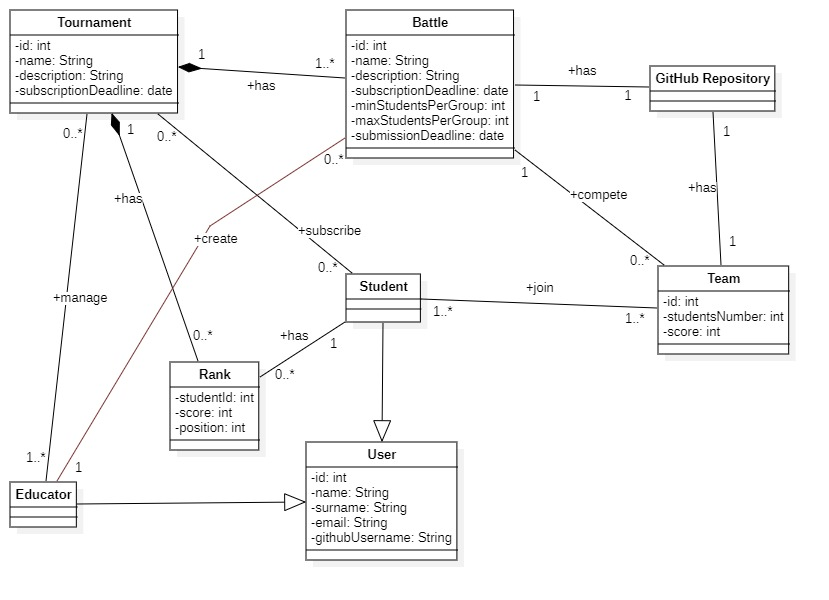
\includegraphics[width=1\linewidth]{DomainClass.jpg}
   \captionof{figure}{Domain class diagram}
  \label{fig:domainclass}
\end{center}
\begin{itemize}
\item There are two types of users: Students and Educators. They both use the system, so they have some attributes in common, such as name, surname and email.
\item Each Educator can manage some Tournaments, which are composed of at least one Battle.
\item Each Tournament has a list of ranks: each rank belongs to a Student that is enrolled into the Tournament.
\item In order to compete in a Battle, Students have to join a Team, whose minimum and maximum number of Students is determined by the Battle the Team participates in.
\item Each Battle is created by an Educator and is associated with a GitHub Repository, which contains information about the battle and the test cases that are going to be used to evaluate Teams’ submissions.
\item Each Team that competes in a Battle will submit their solution using a GitHub Repository.
\end{itemize}
\subsubsection{State Charts}
\begin{center}
    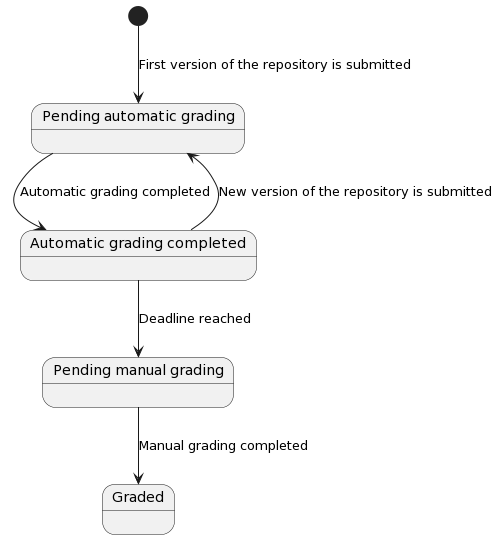
\includegraphics[width=0.5\linewidth]{image4.png}
   \captionof{figure}{State chart that describes the process of managing a tournament}
  \label{fig:managetournament}
\end{center}
\begin{center}
    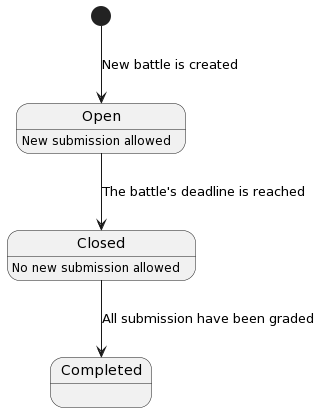
\includegraphics[width=0.5\linewidth]{image10.png}
   \captionof{figure}{State chart that describes the process of managing a battle}
  \label{fig:managebattle}
\end{center}
\begin{center}
    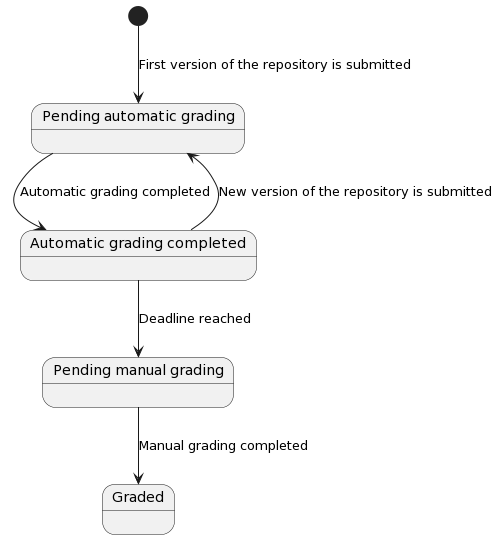
\includegraphics[width=0.5\linewidth]{image6.png}
   \captionof{figure}{State chart that describes the process of managing the grading}
  \label{fig:managegrading}
\end{center}
\begin{center}
    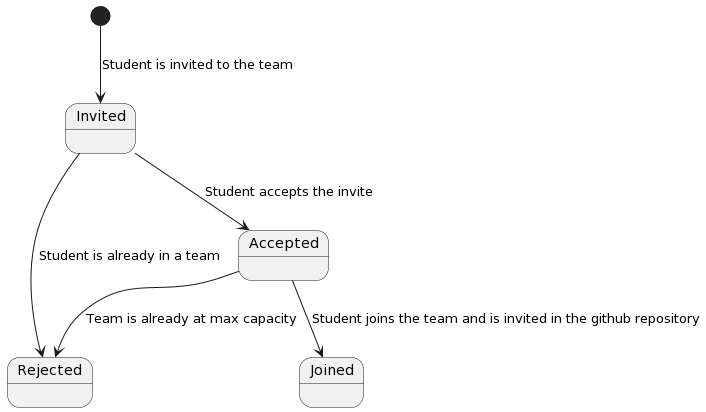
\includegraphics[width=0.8\linewidth]{image15.png}
   \captionof{figure}{State chart that describes the process of managing the invites}
  \label{fig:manageinvites}
\end{center}
\subsection{Product Functions}
\subsubsection{Sign Up and Login}
The sign up and login functions are handled by github, this way the system can manage the user github repositories.
\subsubsection{Create tournament}
This function will be available to educators.
Will allow educators to create tournaments
\subsubsection{Close tournament}
This function will be available to educators.
Will allow educators to close a tournament if they have created it.
\subsubsection{Add educator to tournament}
This function will be available to educators.
Will allow educators to abilitate other educators to create battles for the tournament they create.
\subsubsection{Create battle}
This function will be available to educators.
Will allow educators to create battles
\subsubsection{Grade solution}
This function will be available to educators.
Will allow educators to grade a solution for a battle they have created
\subsubsection{Join tournament}
This function will be available to students.
Will allow students to join tournaments
\subsubsection{Create team}
This function will be available to students.
Will allow students to create team for a battle
\subsubsection{Invite to team}
This function will be available to team leaders.
Will allow students to invite other students in their team
\subsubsection{Accept invite to team}
This function will be available to students.
Will allow students to accept an invite to a team.
\subsubsection{Reject invite to team}
This function will be available to students.
Will allow students to reject invites to join a team
\subsubsection{Check tournament rankings}
This function will be available to students who are participating in the tournament.
Will allow students to check the rankings for that tournament.

\subsection{Users}
\subsubsection{Educator}
A user of the system that creates and manages tournaments and battles.
\subsubsection{Student}
A user of the system that participates in tournaments and battles
\subsection{Assumptions, dependencies and constraints}
\subsubsection{Regulatory policies}
The system doesn’t ask or store any personal data by itself, as github is used for authentication. The system will inherit all restrictions and rules coming from the use of the github api.
\subsubsection{Domain Assumptions}
The following are the assumptions made for the domain. Such assumptions are
properties and/or conditions that the system takes for granted, mostly because they
are out of the control of the system itself, and therefore need to be verified to assure the correct behavior of the system.\\\\
\textbf{[D1]}User has a GitHub account.\\
\textbf{[D2]} User has access to their GitHub account.\\
\textbf{[D3]} Educator inserts the correct information when creating a battle.\\
\textbf{[D4]} Educator provides a correct project structure in the repository for the battle.\\
\textbf{[D5]} Educator provides correct tests in the repository for the battle.\\
\textbf{[D6]} Educator provides correct GitHub actions to run test and static analysts in the repository for the battle.\\
\textbf{[D7]} Student accepts the invitation to the GitHub repository in time.\\
\textbf{[D8]} The solution pushed in the main branch is the solution to be evaluated.\\
\textbf{[D9]} GitHub allows for third parties to manage the user account.\\
\textbf{[D10]} The system is able to connect to GitHub via internet connection.\\
\textbf{[D11]} The system is reachable via the user’s internet connection.\\
\textbf{[D12]} The Student doesn't alterate the repository in such a way that prevents the GitHub actions created by the creator of the battle to be run.\\
\textbf{[D13]} The Educator’s repository is public.\\
\textbf{[D14]} The Student’s repository is public.\\

\newpage
\section{Specific Requirements}

\subsection{External interfaces}
The system will have to interface with:
\begin{itemize}
\item Educators
\item Students
\item Github api
\end{itemize}
\subsubsection{Hardware interfaces}
The system will not have to interface with any particular hardware outside of the users’ devices.
\subsubsection{Software interfaces}
The system will have to interface with:
\begin{itemize}
\item Github authentication system to log in users
\item Github api to manage users repositories
\item Github api to run github the required actions
\end{itemize}
\subsubsection{Communication interfaces}
The system will have to communicate through internet with:
\begin{itemize}
\item Github
\item Users
\end{itemize}

\subsection{Functional requirements}
In the following are specified all the requirements that the system has to fulfill in order to work properly.\\\\

\subsubsection{Requirements index}
\textbf{[R1]} The system allows Students to log in via GitHub.\\
\textbf{[R2]} The system allows Educators to log in via GitHub.\\
\textbf{[R3]} The system allows Educators to create a tournament.\\
\textbf{[R4]} The system allows Educators to view a list of only tournaments they manage.\\
\textbf{[R5]} The system allows Educators to add other Educators to a tournament they manage.\\
\textbf{[R6]} The system allows Educators to view a list of all Educators that manage the tournament they are managing.\\
\textbf{[R7]} The system allows Educators to end a tournament they manage.\\
\textbf{[R8]} The system allows Educators to view a list of Students that are enrolled in a tournament they manage.\\
\textbf{[R9]} The system allows Educators to create a battle in a tournament they manage.\\
\textbf{[R10]} The system allows Educators to view a list of teams that are participating to a battle they have created.\\
\textbf{[R11]} The system allows Educators to view a list of submitted solutions for a battle they have created.\\
\textbf{[R12]} The system allows Educators to view the repository of each solution submitted to a battle they have created.\\
\textbf{[R13]} The system allows Educators to grade a solution for a battle they have created, after the deadline of a battle.\\
\textbf{[R14]} The system allows Educators to see the grade given by the automated tests to a solution of a battle.\\
\textbf{[R15]} The system allows Educators to view the rank scoreboard of a tournament they manage.\\
\textbf{[R16]} The system allows Students to view a list of all available tournaments.\\
\textbf{[R17]} The system allows Students to join a tournament.\\
\textbf{[R18]} The system allows Students to view a list of tournaments they are enrolled in.\\
\textbf{[R19]} The system allows Students to view a list of all available battles of a given tournament.\\
\textbf{[R20]} The system allows Students to create a team for a battle.\\
\textbf{[R21]} The system allows Team Leaders to invite other students to their team.\\
\textbf{[R22]} The system allows Students to view a list of invitations received.\\
\textbf{[R23]} The system allows Students to accept an invite.\\
\textbf{[R24]} The system allows Students to decline an invite.\\
\textbf{[R25]} The system allows Students to view a list of battles they have joined, given a tournament.\\
\textbf{[R26]} The system allows Students to view the description of a battle they are enrolled into.\\
\textbf{[R27]} The system allows Students to view the repository of a battle they are enrolled into.\\
\textbf{[R28]} The system allows Students to view the score of the solution submitted, given a battle, and after the solution has been graded.\\
\textbf{[R29]} The system allows Students to view the rank scoreboard of a tournament they are enrolled in.\\
\textbf{[R30]} The system runs GitHub Actions on battles’ repository.\\
\textbf{[R31]} The system detects when a new version of the main branch is available.\\
\textbf{[R32]} System notifies student they have been invited to a team.\\
\textbf{[R33]} System assign automatic grading.\\
\textbf{[R34]} System notifies students a new battle is available.\\
\textbf{[R35]} System notifies students a new tournament is available. \\
\textbf{[R36]} System notifies a tournament has been closed.\\
\textbf{[R37]} System notifies a student that a battle has ended.\\
\textbf{[R38]} System notifies a team their solution has been graded.\\
\textbf{[R39]} System notifies educators that a new submission is ready to be graded.\\
\textbf{[R40]} System notifies students that the student they have invited to their team has accepted/rejected the invite.\\
\textbf{[R41]} System is able to fork the educator’s repository.\\

\subsubsection{Use Case Diagrams}
In the following are provided the use case diagrams deduced from the scenarios reported in \ref{Formal Analysis}. They help identify the actors interacting with the system and their role within each use case. 

\begin{center}
    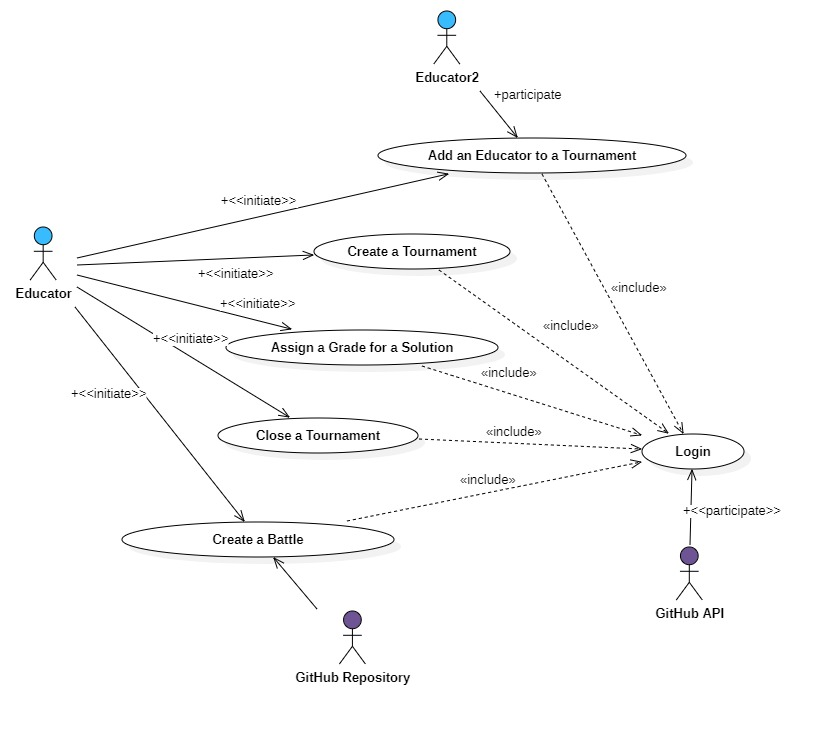
\includegraphics[width=0.8\linewidth]{EducatorUseCase.jpg}
   \captionof{figure}{Educator Use Case Diagram}
  \label{fig:usecaseeducator}
\end{center}

\begin{center}
    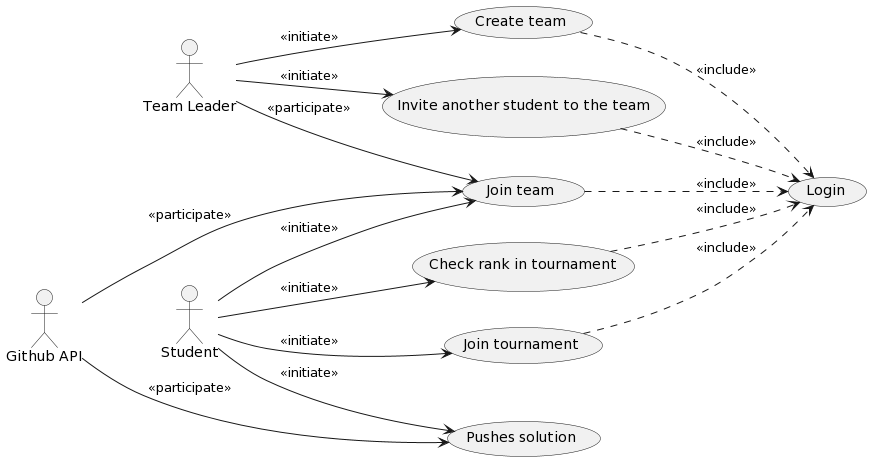
\includegraphics[width=0.9\linewidth]{image19.png}
   \captionof{figure}{Student Use Case Diagram}
  \label{fig:usecasestudent}
\end{center}
\newpage
\subsubsection{Use Cases}

\paragraph{[UC1] Educator creates a tournament}
\begin{center}
\begin{tabular}{|c|m{40em}|}
\hline
Name & Educator creates a tournament\\
\hline
\multirow{2}{4em}{Actors}
& Educator\\
& Students\\
\hline
Entry Condition & The Educator is logged in the system\\
\hline
\multirow{7}{4em}{Event Flow}
& 1- The Educator clicks the “Create Tournament” button\\
& 2- The system shows a form, asking for details about the tournament\\
& 3- The Educator inserts the requested data\\
& 4- The system checks if the data is correct\\
& 5- The Educator clicks the “Confirm tournament creation” button\\
& 6- The system shows a success screen, along with info about the tournament\\
& 7- The system notifies all Students about the new tournament\\
\hline
Exit Condition & The Educator successfully creates a tournament\\
\hline
Exception & 3- The data inserted is not valid. The system returns to Event 2\\
\hline
\end{tabular}
\end{center}

\paragraph{[UC2] Educator adds another educator in a tournament they manage}
\begin{center}
\begin{tabular}{|c|m{40em}|}
\hline
Name & Educator adds another educator in a tournament they manage\\
\hline
\multirow{2}{4em}{Actors}
& Educator\\
& Educator2\\
\hline
Entry Condition & The Educator is logged in the system and is managing a tournament\\
\hline
\multirow{7}{4em}{Event Flow}
& 1- The Educator selects a tournament they manage\\
& 2- The system shows a screen with details about the selected tournament\\
& 3- The Educator clicks the “Add an Educator to tournament” button\\
& 4- The system shows a list of educators that are not currently managing the selected tournament\\
& 5- The Educator selects an Educator to add and clicks the “Add” button\\
& 6- The system notifies Educator2\\
& 7- The website shows a success screen, along with info about the tournament\\
\hline
Exit Condition & The Educator successfully added Educator2 to the tournament\\
\hline
Exception & 5- Educator2 was already added previously\\
\hline
\end{tabular}
\end{center}

\paragraph{[UC3] Educator creates a battle}
\begin{center}
\begin{tabular}{|c|m{40em}|}
\hline
Name & Educator creates a battle\\
\hline
\multirow{2}{4em}{Actors}
& Educator\\
& Students\\
\hline
Entry Condition & The Educator is logged in the system and is managing a tournament\\
\hline
\multirow{9}{4em}{Event Flow}
& 1- The Educator selects a tournament they manage\\
& 2- The system shows a screen with details about the selected tournament\\
& 3- The Educator clicks the “Create battle” button\\
& 4- The system shows a form, asking for details about the battle\\
& 5- The Educator inserts the requested data\\
& 6- The system checks if the data is correct\\
& 7- The Educator clicks the “Confirm battle creation” button\\
& 8- The system shows a success screen, along with info about the battle\\
& 9- The system notifies all Students about the new battle\\
\hline
Exit Condition & The Educator successfully creates a battle\\
\hline
Exception & 5- The data inserted is not valid. The system returns to Event 4\\
\hline
\end{tabular}
\end{center}

\paragraph{[UC4] Educator assigns a grade for a solution}
\begin{center}
\begin{tabular}{|c|m{40em}|}
\hline
Name & Educator assigns a grade for a solution\\
\hline
\multirow{2}{4em}{Actors}
& Educator\\
& Students\\
\hline
Entry Condition &The Educator is logged in the system and is in a battle's management screen. The battle has ended.\\
\hline
\multirow{7}{4em}{Event Flow}
&1- The Educator clicks on the “Evaluate submissions” button\\
&2- The system shows a list of all the submissions ready to be graded\\
&3- The Educator selects the submission they want to evaluate\\
&4- The system shows submission's code and the score of automated tests\\
&5- The Educator selects the grade to assign\\
&6- The system records the grade\\
&7- The system notifies the Students\\
\hline
Exit Condition & The Educator successfully grades a submission\\
\hline
Exception & 5- Invalid grade. The system returns at Event 4\\
\hline
\end{tabular}
\end{center}

\paragraph{[UC5] Educator closes a tournament}
\begin{center}
\begin{tabular}{|c|m{40em}|}
\hline
Name & Educator closes a tournament\\
\hline
\multirow{1}{4em}{Actors}
& Educator\\
\hline
Entry Condition & The Educator is logged in the system and is managing a tournament.\\
\hline
\multirow{5}{4em}{Event Flow}
&1- The Educator selects a tournament they manage\\
&2- The system shows a screen with details about the selected tournament\\
&3- The Educator clicks the “Close tournament” button\\
&4- The system puts the tournament in the “Closed” state\\
&5- On Exit Condition, the system puts the tournament in the “Completed” status.\\
\hline
Exit Condition & All battles are over\\
\hline
\end{tabular}
\end{center}

\paragraph{[UC6] Student joins a tournament}
\begin{center}
\begin{tabular}{|c|m{40em}|}
\hline
Name & Student joins a tournament\\
\hline
\multirow{2}{4em}{Actors}
& Student\\
& Github API\\
\hline
Entry Condition & The Student is logged in the system\\
\hline
\multirow{4}{4em}{Event Flow}
&1- The Student selects an open tournament they are not enrolled in\\
&2- The system shows a screen with details about the selected tournament\\
&3- The Student clicks the "Enroll into tournament” button\\
&4- The system shows a success screen, along with info about the tournament\\
\hline
Exit Condition & The Student successfully enrolled in the tournament\\
\hline
Exception & 1- The student selects an open tournament they are already enrolled in. The system does not show the “Enroll into tournament” button\\
\hline
\end{tabular}
\end{center}

\newpage
\paragraph{[UC7] Student creates a team}
\begin{center}
\begin{tabular}{|c|m{40em}|}
\hline
Name & Student creates a team\\
\hline
\multirow{1}{4em}{Actors}
& Student\\
\hline
Entry Condition & 	\\
\hline
\multirow{5}{4em}{Event Flow}
& 1- The Student selects the tournament\\
& 2- The System returns the view of the tournament\\
& 3- The Student select the battle\\
& 4- The System return the view of the battle\\
& 5- The Student ask the system to create a team\\
& 6- The System checks team name is available\\
& 7- The System checks the student is not in another team for this battle\\
& 8- The System creates a fork of the battle's repository on the student's account\\
& 9- The Team is created\\
\hline
Exit Condition & The Team is created\\
\hline
Exception & 3- The student is already in a team, the team name is not available or the fork cannot be created\\
\hline
\end{tabular}
\end{center}

\paragraph{[UC8] Student joins a team}
\begin{center}
\begin{tabular}{|c|m{40em}|}
\hline
Name & Student joins a team\\
\hline
\multirow{1}{4em}{Actors}
& Student\\
\hline
Entry Condition & The Student is logged in the system, has enrolled in a tournament and has been invited in a team\\
\hline
\multirow{11}{4em}{Event Flow}
& 1- The Student selects the tournament\\
& 2- The System returns the view of the tournament\\
& 3- The Student select the battle\\
& 4- The System return the view of the battle\\
& 5- The Student ask the system for a list of all the invites for the current battle\\
& 6- The System return the invites\\
& 7- The Student accept an invite\\
& 8- The System checks that the student is not in a team for this battle and the team is not at maximum capacity\\
& 9- The Student is invited to the github repository\\
& 10- Team leader is notified\\
& 11- The Student joins the team\\
\hline
Exit Condition & The Student joins the team\\
\hline
\multirow{2}{4em}{Exception}
& 1- The Student is already in a team\\
& 2- The Team is at maximum capacity\\
\hline
\end{tabular}
\end{center}

\newpage
\paragraph{[UC9] Student invites another student to the team}
\begin{center}
\begin{tabular}{|c|m{40em}|}
\hline
Name & Student invites another student to the team\\
\hline
\multirow{2}{4em}{Actors}
& Student\\
& Student2\\
\hline
Entry Condition & The Student is logged in the system, has enrolled in a tournament and is part of a team\\
\hline
\multirow{10}{4em}{Event Flow}
& 1- The Student selects the tournament\\
& 2- The System returns the view of the tournament\\
& 3- The Student select the battle\\
& 4- The System return the view of the battle\\
& 5- The Student ask the system for a list of all available students for this battle\\\
& 7- The System return the list\\
& 7- The Student select a student\\
& 8- The System checks that the student is the team leader\\
& 9- The System checks that the invited student is not in a team for this battle and the team is not at maximum capacity\\
& 10- The System sends the invite\\
\hline
Exit Condition & The Invite is sent\\
\hline
\multirow{3}{4em}{Exception}
& 1- The invited student is already in a team\\
& 2- The Team is at maximum capacity\\
& 3- The Student is not team leader\\
\hline
\end{tabular}
\end{center}

\paragraph{[UC10] Student checks his rank for a tournament they are participating in}
\begin{center}
\begin{tabular}{|c|m{40em}|}
\hline
Name & Student checks his rank for a tournament they are participating in\\
\hline
\multirow{1}{4em}{Actors}
& Student\\
\hline
Entry Condition & The Student is logged in the system, has enrolled in a tournament\\
\hline
\multirow{4}{4em}{Event Flow}
& 1- The Student selects the tournament\\
& 2- The System returns the view of the tournament\\
& 3- The Student ask the system for the rankings\\
& 4- The System return the rankings\\
\hline
Exit Condition & The System return the rankings\\
\hline
\end{tabular}
\end{center}

\paragraph{[UC11] A team pushes their solution to GitHub}
\begin{center}
\begin{tabular}{|c|m{40em}|}
\hline
Name & A team pushes their solution to GitHub\\
\hline
\multirow{2}{4em}{Actors}
& Student\\
& Github API\\
\hline
Entry Condition & The Student pushes a new version on the main branch in a repository associated with a team\\
\hline
\multirow{5}{4em}{Event Flow}
& 1- The Student pushes a new version in the main branch\\
& 2- The Github API signals to the system that a new submission is available\\
& 3- The System checks if the team has the minimum number of members\\
& 4- The System runs the associated github actions retrieving the output\\
& 5- The System completes the automatic grading of the solution\\
\hline
Exit Condition & The System completes the automatic grading of the solution\\
\hline
Exception & 1- The team has not the minimum number of members\\
\hline
\end{tabular}
\end{center}

\newpage
\paragraph{[UC12] Battle's deadline is reached}
\begin{center}
\begin{tabular}{|c|m{40em}|}
\hline
Name & Battle's deadline is reached\\
\hline
\multirow{1}{4em}{Actors}
& Educator\\
\hline
Entry Condition & The System detects that a battle's deadline has been reached\\
\hline
\multirow{3}{4em}{Event Flow}
&1- The System changes the status of the battle to closed\\
&2- The System notifies the students that the battle is closed\\
&3- The System notifies the educator that they need to grade the solutions of this battle\\
\hline
Exit Condition & The System notifies the educator that they need to grade the solutions of this battle\\
\hline
\end{tabular}
\end{center}

\paragraph{[UC13] Login of a User}
\begin{center}
\begin{tabular}{|c|m{40em}|}
\hline
Name & Login of a User\\
\hline
\multirow{2}{4em}{Actors}
& User\\
& Github API\\
\hline
Entry Condition & The user logs in the system\\
\hline
\multirow{8}{4em}{Event Flow}
& 1- The User ask the system to log in\\
& 2- The System redirects the user to the Github authentication\\
& 3- The User completes the Github authentication\\
& 4- The Github api returns an access token to the user\\
& 5- The User ask the system to log in with the access token\\
& 6- The System ask the Github api to verify the access token\\
& 7- The Github api returns that the token is valid\\
& 8- The System confirms to the user that they are logged in\\
\hline
Exit Condition & The user is logged in the system\\
\hline
Exception & 3- The access token is not valid\\
\hline
\end{tabular}
\end{center}
\newpage
\subsubsection{Sequence diagrams}

\begin{center}
    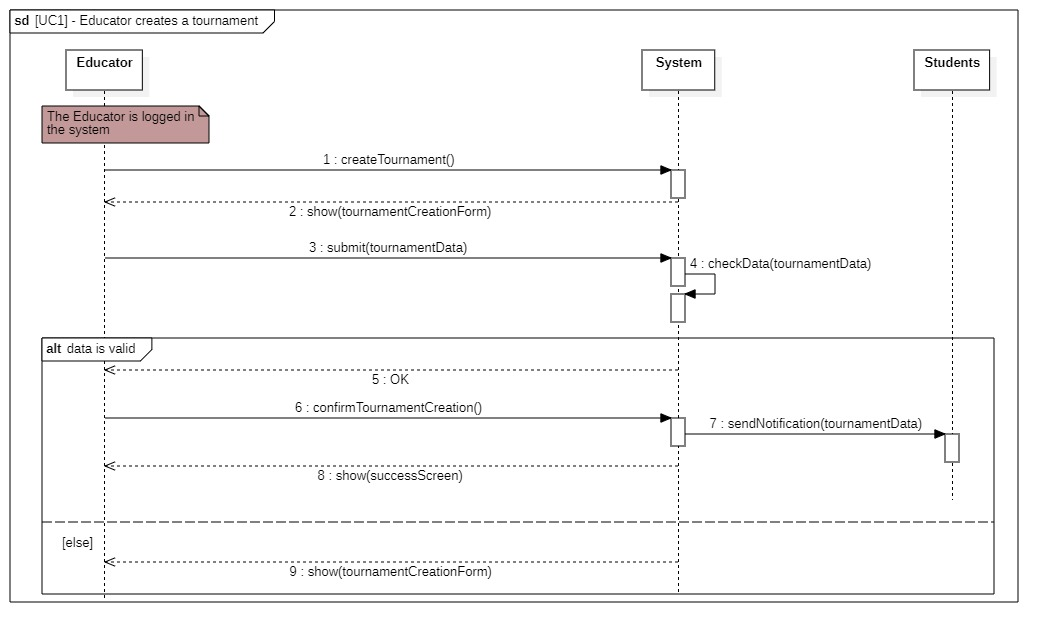
\includegraphics[width=\linewidth]{uc1.jpg}
   \captionof{figure}{[UC1] Educator creates a tournament}
  \label{fig:uc1}
\end{center}

\begin{center}
    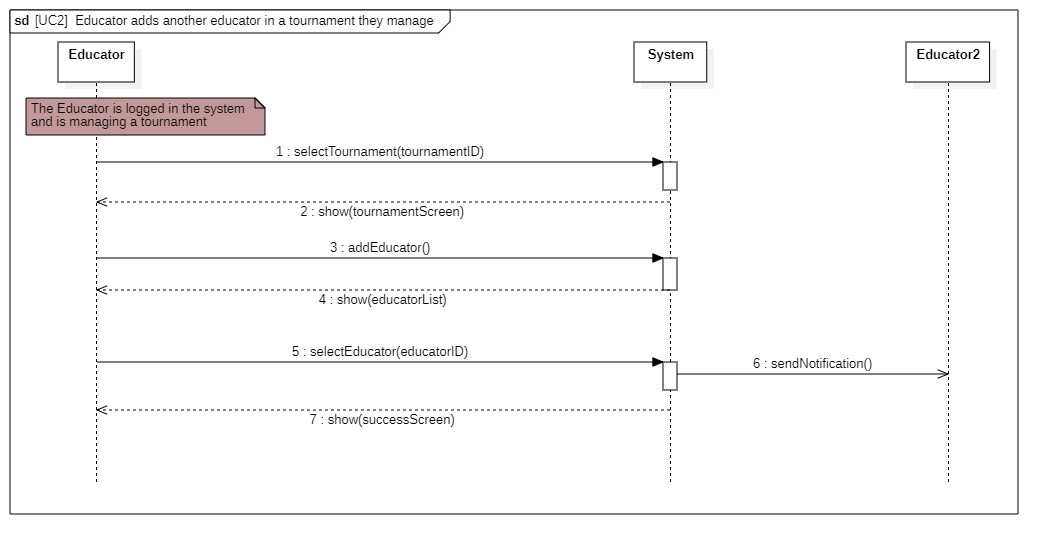
\includegraphics[width=\linewidth]{uc2.jpg}
   \captionof{figure}{[UC2] Educator adds another educator in a tournament they manage}
  \label{fig:uc2}
\end{center}

\begin{center}
    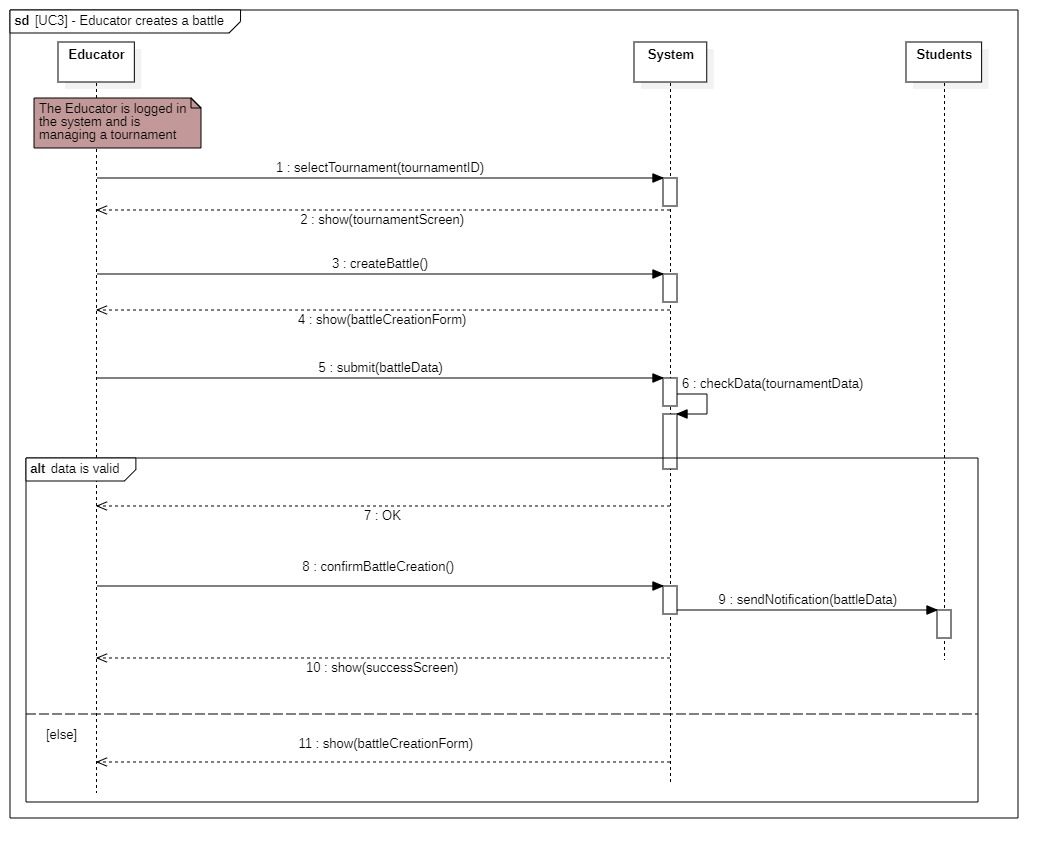
\includegraphics[width=\linewidth]{uc3.jpg}
   \captionof{figure}{[UC3] Educator creates a battle}
  \label{fig:uc3}
\end{center}

\begin{center}
    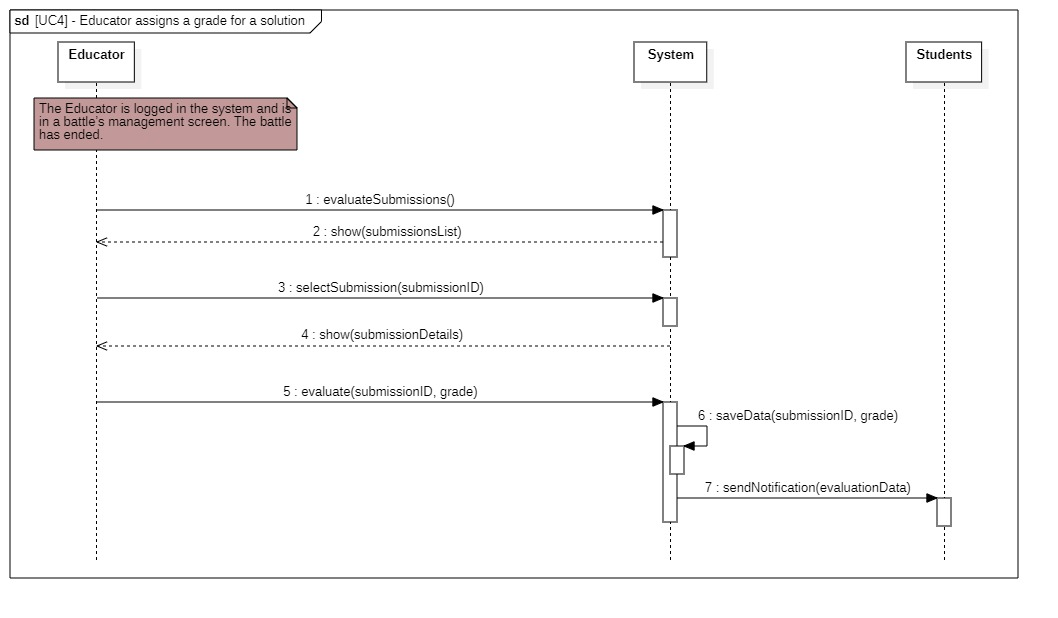
\includegraphics[width=\linewidth]{uc4.jpg}
   \captionof{figure}{[UC4] Educator assigns a grade for a solution}
  \label{fig:uc4}
\end{center}

\begin{center}
    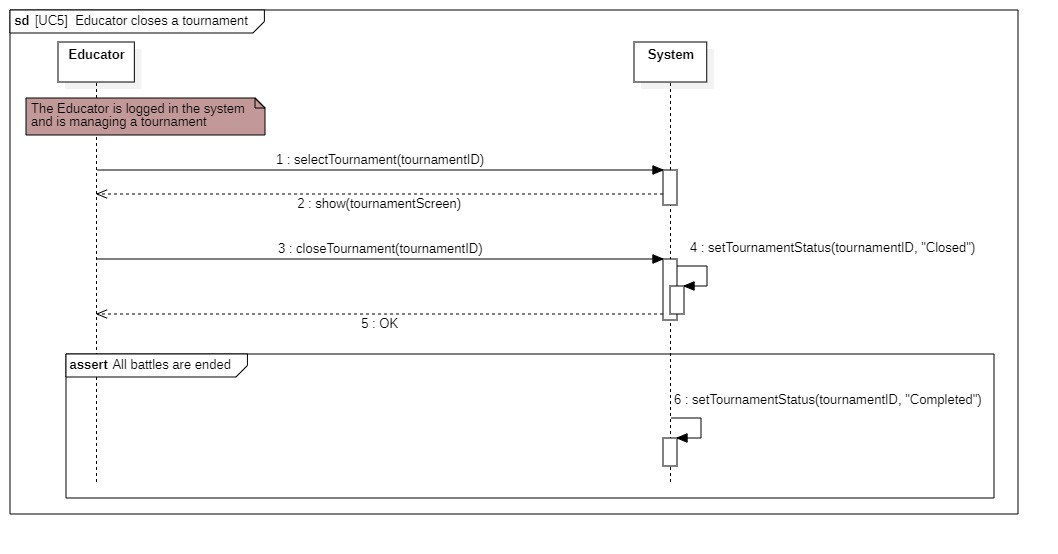
\includegraphics[width=\linewidth]{uc5.jpg}
   \captionof{figure}{[UC5] Educator closes a tournament}
  \label{fig:uc5}
\end{center}

\begin{center}
    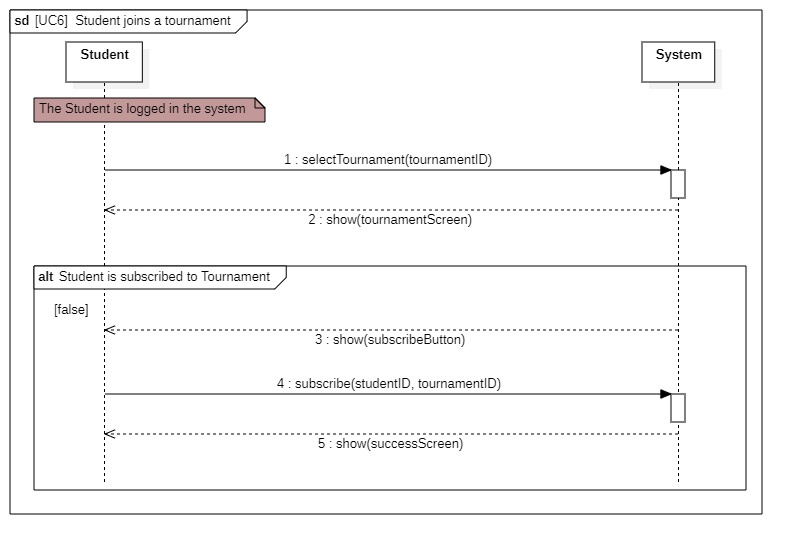
\includegraphics[width=\linewidth]{uc6.jpg}
   \captionof{figure}{[UC6] Student joins a tournament}
  \label{fig:uc6}
\end{center}
\begin{center}
    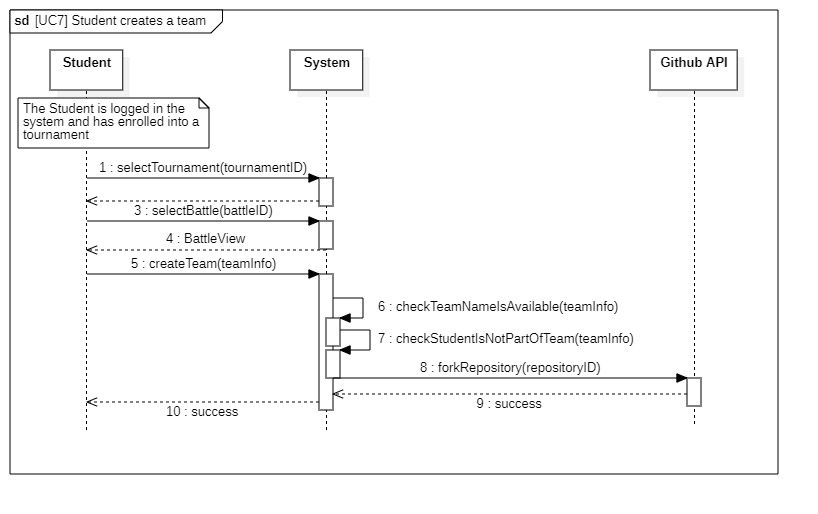
\includegraphics[width=\linewidth]{uc7.jpg}
   \captionof{figure}{[UC7] Student creates a team}
  \label{fig:uc7}
\end{center}

\begin{center}
    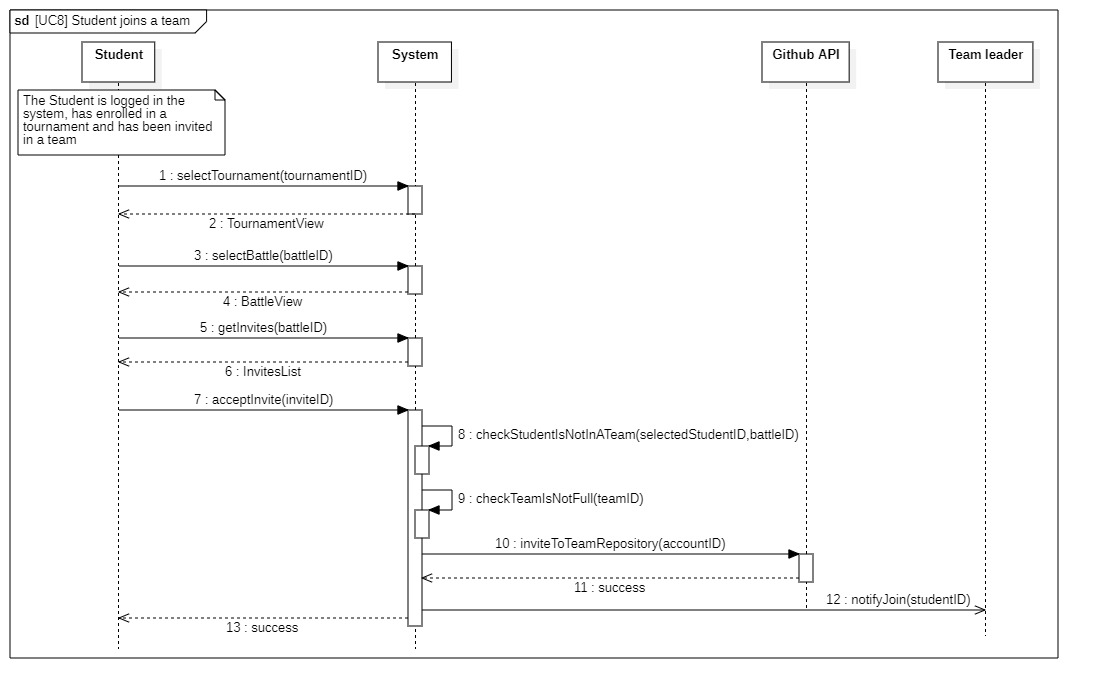
\includegraphics[width=\linewidth]{uc8.jpg}
   \captionof{figure}{[UC8] Student joins a team}
  \label{fig:uc8}
\end{center}

\begin{center}
    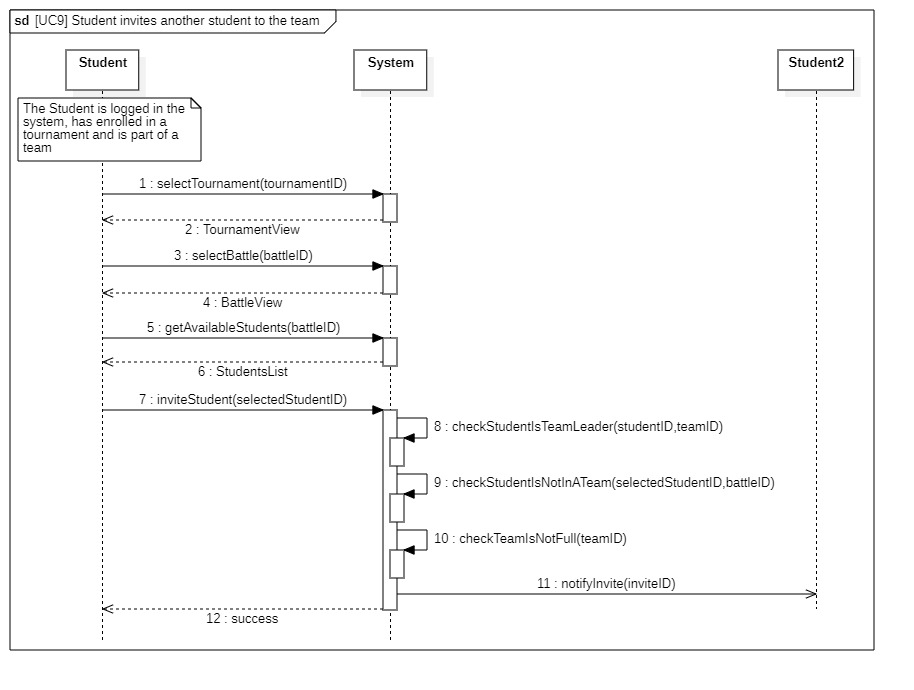
\includegraphics[width=\linewidth]{uc9.jpg}
   \captionof{figure}{[UC9] Student invites another student to the team}
  \label{fig:uc9}
\end{center}

\begin{center}
    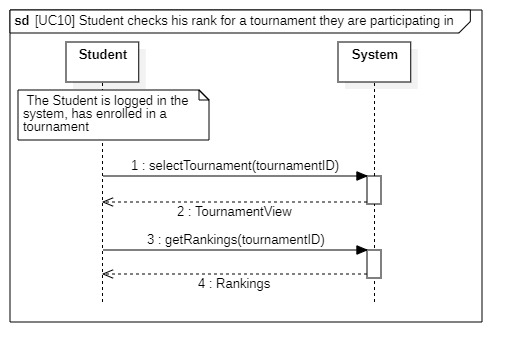
\includegraphics[width=\linewidth]{uc10.jpg}
   \captionof{figure}{[UC10] Student checks his rank for a tournament they are participating in}
  \label{fig:uc10}
\end{center}

\begin{center}
    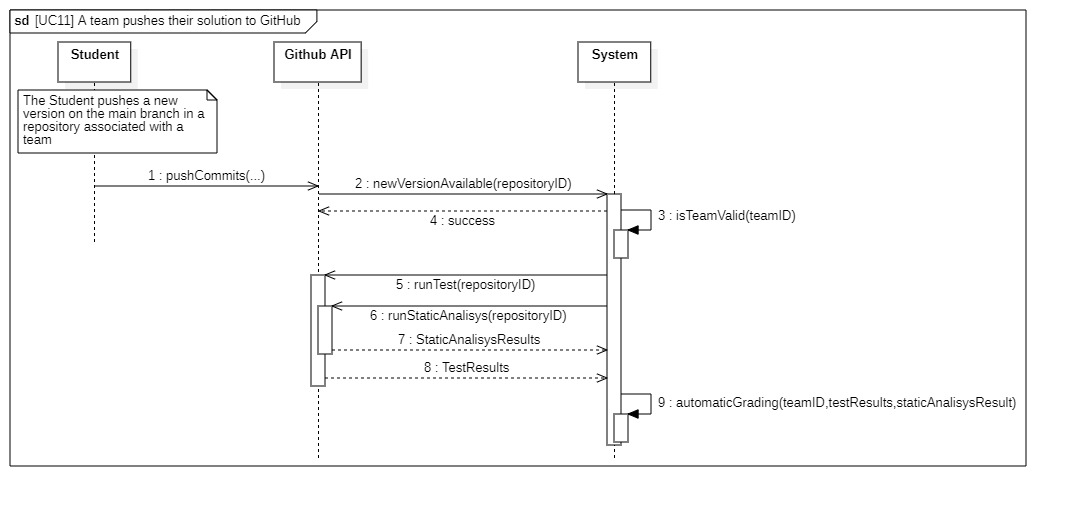
\includegraphics[width=\linewidth]{uc11.jpg}
   \captionof{figure}{[UC11] A team pushes their solution to GitHub}
  \label{fig:uc11}
\end{center}

\begin{center}
    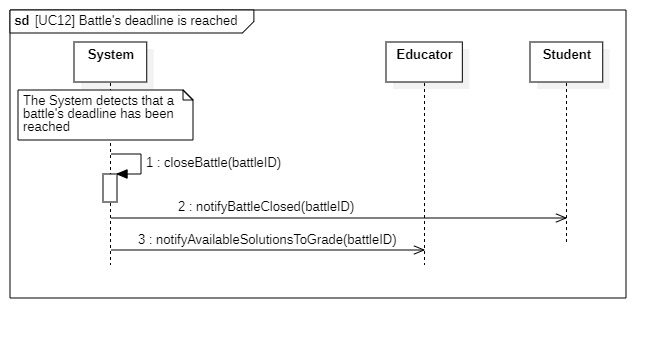
\includegraphics[width=\linewidth]{uc12.jpg}
   \captionof{figure}{[UC12] Battle’s deadline is reached}
  \label{fig:uc12}
\end{center}

\begin{center}
    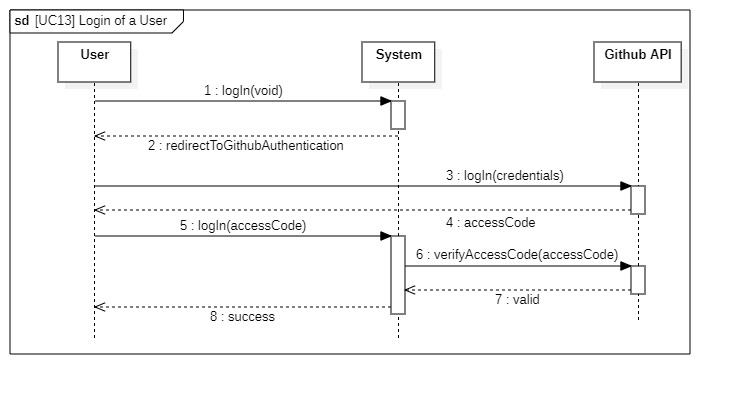
\includegraphics[width=\linewidth]{uc13.jpg}
   \captionof{figure}{[UC13] - Login of a User}
  \label{fig:uc13}
\end{center}

\subsubsection{Requirements mapping}

\paragraph{[G1] Educator is able to create and manage a tournament}
\begin{center}
\begin{tabular}{|m{20em}|m{20em}|}
\hline
& \\
{[R2]} The system allows Educators to log in via GitHub. &
{[D1]} User has a GitHub account.\\
{[R3]} The system allows Educators to create a tournament. &
{[D2]} User has access to their GitHub account.\\
{[R4]} The system allows Educators to view a list of only tournaments they manage. &
[D10] The system is able to connect to GitHub via internet connection.\\
{[R6]} The system allows Educators to view a list of all Educators that manage the tournament they are managing. &
[D11] The system is reachable via the user’s internet connection.\\
{[R7]} The system allows Educators to end a tournament they manage. & \\
{[R8]} The system allows Educators to view a list of Students that are enrolled in a tournament they manage. & \\
{[R15]} The system allows Educators to view the rank scoreboard of a tournament they manage. & \\
{[R35]} System notifies students a new tournament is available.  & \\
{[R36]} System notifies a tournament has been closed. & \\
\hline
\end{tabular}
\end{center}

\paragraph{[G2] Educator is able to allow other educators to manage their tournament}
\begin{center}
\begin{tabular}{|m{20em}|m{20em}|}
\hline
& \\
{[R2]} The system allows Educators to log in via GitHub. &
{[D1]} User has a GitHub account.\\
{[R4]} The system allows Educators to view a list of only tournaments they manage. &  \\
{[D2]} User has access to their GitHub account.\\
{[R5]} The system allows Educators to add other Educators to a tournament they manage. &  \\
{[D10]} The system is able to connect to GitHub via internet connection.\\
{[R6]} The system allows Educators to view a list of all Educators that manage the tournament they are managing. &  \\
{[D11]} The system is reachable via the user's internet connection.\\
\hline
\end{tabular}
\end{center}

\paragraph{[G3] Educator is able to create and manage code battles for a tournament they are involved in
}
\begin{center}
\begin{tabular}{|m{20em}|m{20em}|}
\hline
& \\
{[R2]} The system allows Educators to log in via GitHub. &
{[D1]} User has a GitHub account.\\
{[R4]} The system allows Educators to view a list of only tournaments they manage. &
{[D2]} User has access to their GitHub account.\\
{[R9]} The system allows Educators to create a battle in a tournament they manage. &
{[D3]} Educator inserts the correct information when creating a battle.\\
{[R10]} The system allows Educators to view a list of teams that are participating to a battle they have created. &
{[D4]} Educator provides a correct project structure in the repository for the battle.\\
{[R11]} The system allows Educators to view a list of submitted solutions for a battle they have created. &
{[D5]} Educator provides correct tests in the repository for the battle.\\
{[R12]} The system allows Educators to view the repository of each solution submitted to a battle they have created. &
{[D6]} Educator provides correct GitHub actions to run test and static analysts in the repository for the battle.\\
{[R30]} The system runs GitHub Actions on battles’ repository. &
{[D9]} GitHub allows for third parties to manage the user account.\\
{[R34]} System notifies students a new battle is available. &
{[D10]} The system is able to connect to GitHub via internet connection.\\
{[R37]} System notifies a student a battle is ended. &
{[D11]} The system is reachable via the user’s internet connection.\\
\hline
\end{tabular}
\end{center}

\paragraph{[G4] Any user is able to authenticate with their GitHub account}
\begin{center}
\begin{tabular}{|m{20em}|m{20em}|}
\hline
& \\
{[R1]} The system allows Students to log in via GitHub. & 
{[D1]} User has a GitHub account.\\
{[R2]} The system allows Educators to log in via GitHub. & 
{[D2]} User has access to their GitHub account.\\
& {[D10]} The system is able to connect to GitHub via internet connection.\\
& {[D11]} The system is reachable via the user’s internet connection.\\
\hline
\end{tabular}
\end{center}

\paragraph{[G5] Student is able to enroll in tournament and join/create a team.}
\begin{center}
\begin{tabular}{|m{20em}|m{20em}|}
\hline
& \\
{[R1]} The system allows Students to log in via GitHub. & 
{[D1]} User has a GitHub account.\\
{[R16]} The system allows Students to view a list of all available tournaments. & 
{[D2]} User has access to their GitHub account.\\
{[R17]} The system allows Students to join a tournament. & 
{[D7]} Student accepts the invitation to the GitHub repository in time.\\
{[R34]} System notifies students a new battle is available. & 
{[D9]} GitHub allows for third parties to manage the user account.\\
{[R19]} The system allows Students to view a list of all available battles of a given tournament. & 
{[D10]} The system is able to connect to GitHub via internet connection.\\
{[R20]} The system allows Students to create a team for a battle. & 
{[D11]} The system is reachable via the user's internet connection.\\
{[R21]} The system allows Team Leaders to invite other students to their team. & 
{[D13]} The Educator's repository is public.\\
{[R22]} The system allows Students to view a list of invitations received. & 
\\
{[R23]} The system allows Students to accept an invite. & 
\\
{[R24]} The system allows Students to decline an invite. & 
\\
{[R25]} The system allows Students to view a list of battles they have joined, given a tournament. & 
\\
{[R34]} System notifies students a new battle is available. & 
\\
{[R32]} System notifies student they have been invited to a team. & 
\\
{[R35]} System notifies students a new tournament is available.  & 
\\
{[R40]} System notifies students that the student they have invited to their team has accepted/rejected the invite. & 
\\
{[R41]} System is able to fork the educator’s repository. & 
\\
\hline
\end{tabular}
\end{center}

\paragraph{[G6] Any Team participating in a battle is able to submit a solution.}
\begin{center}
\begin{tabular}{|m{20em}|m{20em}|}
\hline
& \\
{[R13]} The system allows Educators to grade a solution for a battle they have created, after the deadline of a battle. & 
{[D1]} User has a GitHub account.\\
{[R26]} The system allows Students to view the description of a battle they are enrolled into. & 
{[D2]} User has access to their GitHub account.\\
{[R27]} The system allows Students to view the repository of a battle they are enrolled into. & 
{[D4]} Educator provides a correct project structure in the repository for the battle.\\
{[R30]} The system runs GitHub Actions on battles' repository. & 
{[D5]} Educator provides correct tests in the repository for the battle.\\
{[R31]} The system detects when a new version of the main branch is available. & 
{[D6]} Educator provides correct GitHub actions to run test and static analysts in the repository for the battle.\\
{[R33]} System assign automatic grading. & 
{[D8]} The solution pushed in the main branch is the solution to be evaluated.\\
& {[D9]} GitHub allows for third parties to manage the user account. \\
& {[D10]} The system is able to connect to GitHub via internet connection. \\
& {[D11]} The system is reachable via the user’s internet connection. \\
& {[D12]} The Student doesn't alterate the repository in such a way that prevents the GitHub actions created by the creator of the battle to be run. \\

\hline
\end{tabular}
\end{center}


\paragraph{[G7]Students are able to see their current rank and score in the tournaments they are taking part.}
\begin{center}
\begin{tabular}{|m{20em}|m{20em}|}
\hline
& \\
{[R1]} The system allows Students to log in via GitHub. &
{[D1]} User has a GitHub account.\\
{[R18]} The system allows Students to view a list of tournaments they are enrolled in. &
{[D2]} User has access to their GitHub account.\\
{[R29]} The system allows Students to view the rank scoreboard of a tournament they are enrolled in. &
{[D10]} The system is able to connect to GitHub via internet connection.\\
{[R36]} System notifies a tournament has been closed. &
{[D11]} The system is reachable via the user's internet connection.\\
{[R37]} System notifies a student a battle has ended. & \\
\hline
\end{tabular}
\end{center}

\paragraph{[G8] Educators are able to see Student's current rank and score in the tournaments they are involved in.}
\begin{center}
\begin{tabular}{|m{20em}|m{20em}|}
\hline
& \\
{[R2]} The system allows Educators to log in via GitHub. &
{[D1]} User has a GitHub account.\\
{[R4]} The system allows Educators to view a list of only tournaments they manage. &
{[D2]} User has access to their GitHub account.\\
{[R15]} The system allows Educators to view the rank scoreboard of a tournament they manage. &
{[D10]} The system is able to connect to GitHub via internet connection.\\
{[R38]} System notifies a team their solution has been graded. &
{[D11]} The system is reachable via the user's internet connection.\\
\hline
\end{tabular}
\end{center}

\paragraph{[G9] Educators are able to assign a grade to solutions submitted by Teams subscribed to a Battle created by the Educator.}
\begin{center}
\begin{tabular}{|m{20em}|m{20em}|}
\hline
& \\
{[R2]} The system allows Educators to log in via GitHub. & 
{[D1]} User has a GitHub account.\\
{[R4]} The system allows Educators to view a list of only tournaments they manage. & 
{[D2]} User has access to their GitHub account.\\
{[R11]} The system allows Educators to view a list of submitted solutions for a battle they have created. & 
{[D10]} The system is able to connect to GitHub via internet connection.\\
{[R12]} The system allows Educators to view the repository of each solution submitted to a battle they have created. & 
{[D11]} The system is reachable via the user's internet connection.\\
{[R13]} The system allows Educators to grade a solution for a battle they have created, after the deadline of a battle. & 
{[D8]} The solution pushed in the main branch is the solution to be evaluated.\\
{[R14]} The system allows Educators to see the grade given by the automated tests to a solution of a battle. & 
{[D9]} GitHub allows for third parties to manage the user account.\\
{[R28]} The system allows Students to view the score of the solution submitted, given a battle, and after the solution has been graded. & 
{[D12]} The Student doesn't alterate the repository in such a way that prevents the GitHub actions created by the creator of the battle to be run.\\
{[R33]} System assign automatic grading. & 
{[D14]} The Student's repository is public.\\
{[R39]} System notifies educator that a new  &  \\
\hline
\end{tabular}
\end{center}

\subsubsection{Performance requirements}
The system needs to be able to serve multiple users at the same time and to manage the grading and tracking of solutions in a manner that doesn’t jeopardize the outcome of a battle.


\subsubsection{Design Constraints}
Being dependent on github the system will be able to manage users repositories and data only according to github api.\\
The system performance however is strictly connected with the github action performance.

\subsection{Software System Attributes}

\subsubsection{Reliability}
The system has to be able to run continuously without any interruptions for long periods. To be fault-tolerant the system backend deployment must take advantage of some sort of replication and redundancy. The system has to have offline backups of the data storage to exploit in disaster recovery after a data loss.					
\subsubsection{Availability}					
Given the fact that CodeKataBattle is not an emergency service or anything related to critical situations, the system must provide availability of 99%. This means that the downtime of the system has to be 3.65 days per year.		
\subsubsection{Security}					
The system doesn’t store sensitive personal information about users, since every user of the system authenticates via GitHub. To communicate over the internet CodeKataBattle must use some sort of encryption to avoid traffic sniffing and spoofing, thus avoiding cheating attacks and guaranteeing privacy and consistency.				
\subsubsection{Maintainability}				
The system must guarantee a high level of maintainability. Appropriate design patterns should be used, together with good standards. The code must be well documented and hard-coding must be avoided. A testing routine has to be provided and it has to cover at least 85% of the entire codebase, excluding interface code.				
\subsubsection{Portability}			
The web application must run on any OS (like Windows, Mac OS, Linux, etc) that supports a web browser.
Self hosted component of the stystem must be able to run on a Linux server.

\newpage
\section{Formal Analysis}
With alloy we can formally verify that the constraints of the system are coherent and true

\subsection{Signatures}
With the signatures we describe entities that are part of the system with their relationships.
\begin{lstlisting}
  sig Student{}
  sig Educator{}
  
  sig Team{
      team_mates: some Student,
      battle: one Battle
  }
  
  sig Battle{
      creator: one Educator,
      tournament: one Tournament,
      teams: set Team,
  }
  
  sig Tournament{
      creator: one Educator,
      allowed_educators: set Educator,
      battles: set Battle,
      students: set Student
  }
\end{lstlisting}

\subsection{Predicates}
\begin{lstlisting}[
  breaklines=true,
  postbreak=\mbox{{$\hookrightarrow$}\space}]
pred CanCreateBattles[e : Educator, t:Tournament]{
    e in t.allowed_educators
}

pred CreatedTournament[e : Educator, t:Tournament]{
    t.creator = e
}

pred CanCloseTournament[e : Educator, t:Tournament]{
    t.creator = e
}

pred CanGradeSolutions[e: Educator, b: Battle]{
    e = b.creator
}

pred StudentInBattle[s: Student, b: Battle]{
    some t: b.teams | s in t.team_mates
}
\end{lstlisting}

\subsection{Facts}
\begin{lstlisting}[
  breaklines=true,
  postbreak=\mbox{{$\hookrightarrow$}\space}]
fact CreatorIsAllowedEdcator{
    all e: Educator | all t: Tournament | t.creator = e implies e in t.allowed_educators
}

fact BattleIsPartOfTournament{
    all t: Tournament | all b: Battle | b.tournament = t iff b in t.battles
}

fact TeamIsPartOfBattle{
    all t: Team | all b: Battle | t.battle = b iff t in b.teams
}

fact StudentInTeamHasToBeEnrolled{
    all t: Team | all s: Student | s in t.team_mates implies s in t.battle.tournament.students
}

fact StudentCanOnlyBeInOneTeamPerBattle{
	all disj t1,t2: Team | t1.battle = t2.battle implies no (t1.team_mates & t2.team_mates)
}
\end{lstlisting}

\subsection{Assertions}
\begin{lstlisting}[
  breaklines=true,
  postbreak=\mbox{{$\hookrightarrow$}\space}]
assert CreatorCanManageTournament{
    all e: Educator | all t: Tournament | CreatedTournament[e,t] implies (CanCloseTournament[e,t] and CanCreateBattles[e,t])
}

assert NoCommonTeammatesInBattle{
        all s: Student | all disj t1,t2: Team | (s in t1.team_mates and s in t2.team_mates) implies not (t1.battle = t2.battle)
}
\end{lstlisting}

\subsection{Istance}
\begin{center}
  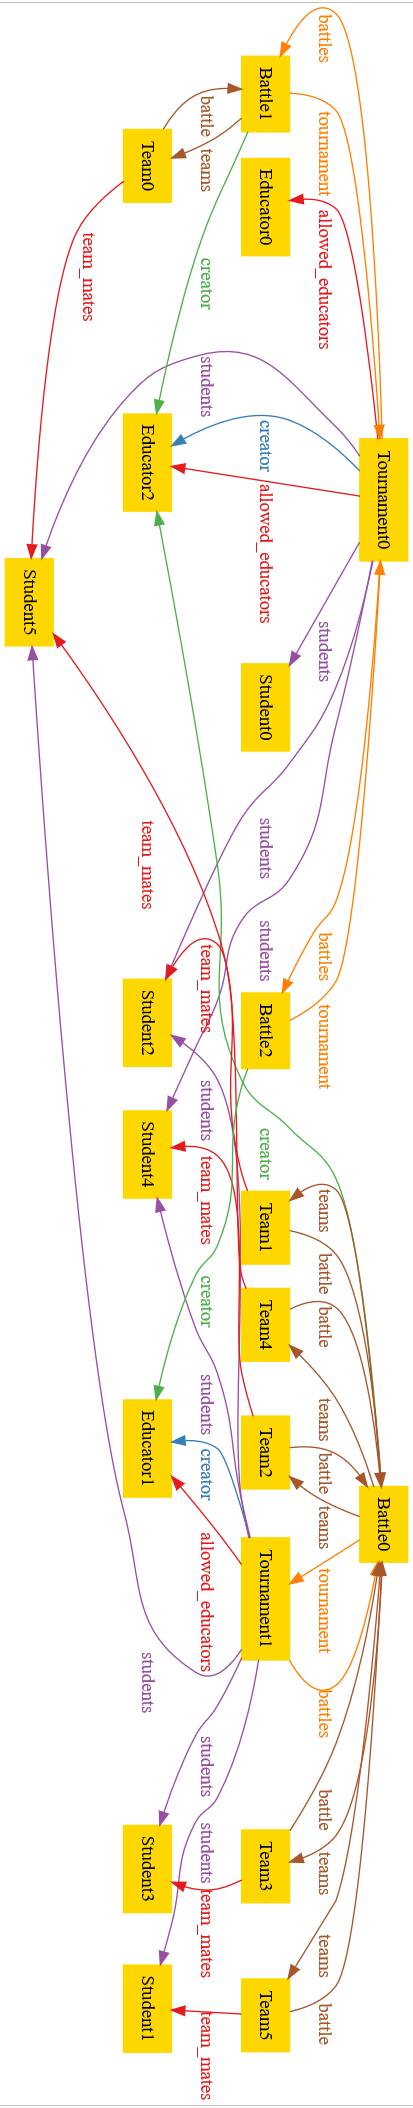
\includegraphics[width=0.25\linewidth]{istance.png}
 \captionof{figure}{example of valid instance of the system}
\label{fig:uc13}
\end{center}

\newpage
\section{Effort Spent}
\begin{center}
\begin{tabular}{||l|c|c|c|c||}
\hline
Student & Section 1 & Section 2 & Section 3 & Section 4
\\
\hline
Merlino Lorenzo & 3h & 4h & 5h & 3h
\\
\hline
Iodice Andrea & 3h & 5h & 6h & ?h
\\
\hline
\end{tabular}
\end{center}

\newpage
\section{References}
\begin{itemize}
\item UML diagrams: plantUML, starUML
\item Alloy: vscode, alloytools
\end{itemize}
\end{document}